\chapter{Introduction}
% \section{Main Idea}
We are living in the digital era where a mobile phone is everybody's best friend. The Internet is all around us, and it almost feels like a commodity. People consider it a fundamental human right, like water. They are used to be online every day from the moment they open their eyes until the moment they shut them again at night. Everyone is obsessed with immediate access to information. That is why mobile applications are so significant these days. They provide a quick way of finding the data that we are interested in. We live quickly, and we want to simplify and speed up some tasks. That is where mobile programs come in handy. Opening a web browser, entering an address and logging in takes lots of time compared to a single click on an app icon.

Not so long ago, mobile phones allowed only for calls and messages. After some time, simple applications started to appear. Most of them were mobile games that you could download on your computer and transfer to your device. You could also download them using, then very slow, Internet connection and WAP protocol. Currently, there are stores where users can search for apps by name, type, or functionalities. It is very comfortable because customers can find everything that they want in one place. It is also convenient for developers because they get access to a bigger audience when publishing their program on such a platform.

On the other hand, we could use our computers for all tasks. The problem is that they are massive and heavy in comparison to phones. People carry the latter with them everywhere. They allow us to connect to the Internet, use built-in GPS, gyroscope, Bluetooth, cameras, and more. To use computers, also laptops, we have to sit down, turn them on, sometimes log in, only then we can order some things or browse the Internet. That is why there is a need for mobile applications. They allow us to pay phone bills, order clothes, play games, and chat with friends whenever we go. It does not matter if we are traveling in a metro or lying on a couch in a living room.

There are some places where the Internet connection is extremely slow, unstable, or it does not exist. When this happens, mobile applications should be ready to handle the situation. They download data when there is a connection and then store it locally. Thanks to this, users do not have to have constant access to the World Wide Web. Sometimes a service from which our app is getting all the data is down. Saving information on a device allows users to use the app even though the server is inaccessible.

Some universities have their mobile applications allowing students to browse news feed from their faculty and university, see calendars, grades, and other information. They let users send and check emails from other students and lecturers. Some educational institutions do not have mobile apps. They use systems that can be accessed only via web browsers. Wrocław University of Science and Technology also has one. It is not optimized for mobile devices, and some functionalities are difficult to access from a phone. The service also gets unavailable from time to time, returning an error message. Usually, when many people try to access it at the same time, for example, during an examination session. That has been an inspiration for the project described in the thesis. It is designed to improve the mobile experience and allow users to access the data when the system is offline.

% TODO - refer to other solutions offering a required set of functions - I've found only these two applications

Two similar solutions exist in Poland. Both of them are represented in Fig.~\ref{fig:similiar-solutions}. One was explicitly created for the University of Warsaw (see Fig.~\ref{fig:similiar-solutions}a). We draw inspiration from it to include some functionalities like news feed and mailbox in our project. Unlike the first app, the second one (see Fig.~\ref{fig:similiar-solutions}b) can show data for more than one university. Users have to choose what university they attend, and then they can see their calendar, grades, and some other data from the chosen university system. This is what we wanted to achieve while designing our application. Most of our attention went to creating a simple and extensible API. The program represented in the document was designed to provide better user experience than the second solution described here, and it is supposed to be easily expendable by YAML files, new widgets, and views.

% TODO - ask if I can use these graphics and how to link them
\begin{figure}[htb]
    \centering
    \begin{tabular}{@{}ll@{}}
        a) & b) \\
        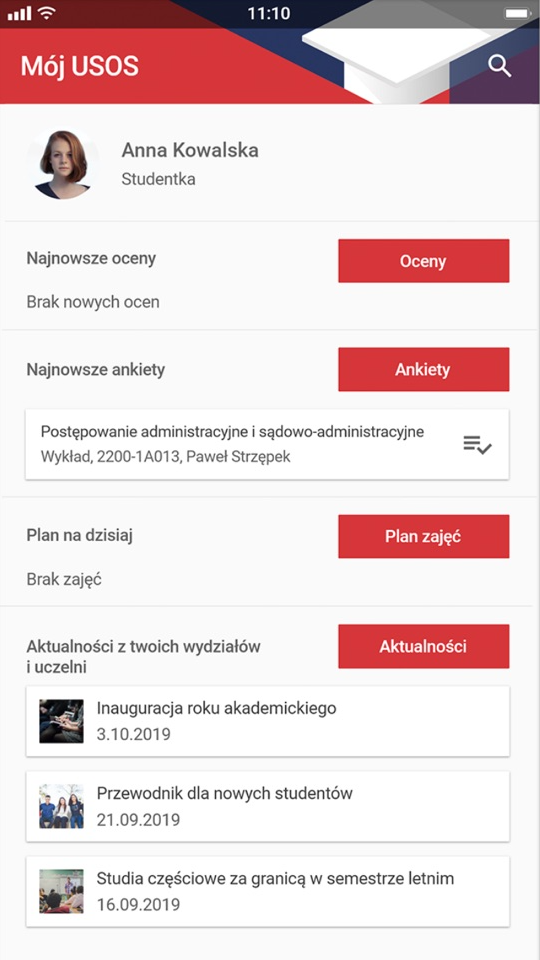
\includegraphics[width=0.425\textwidth]{fig01/mobilny-usos.png} &
        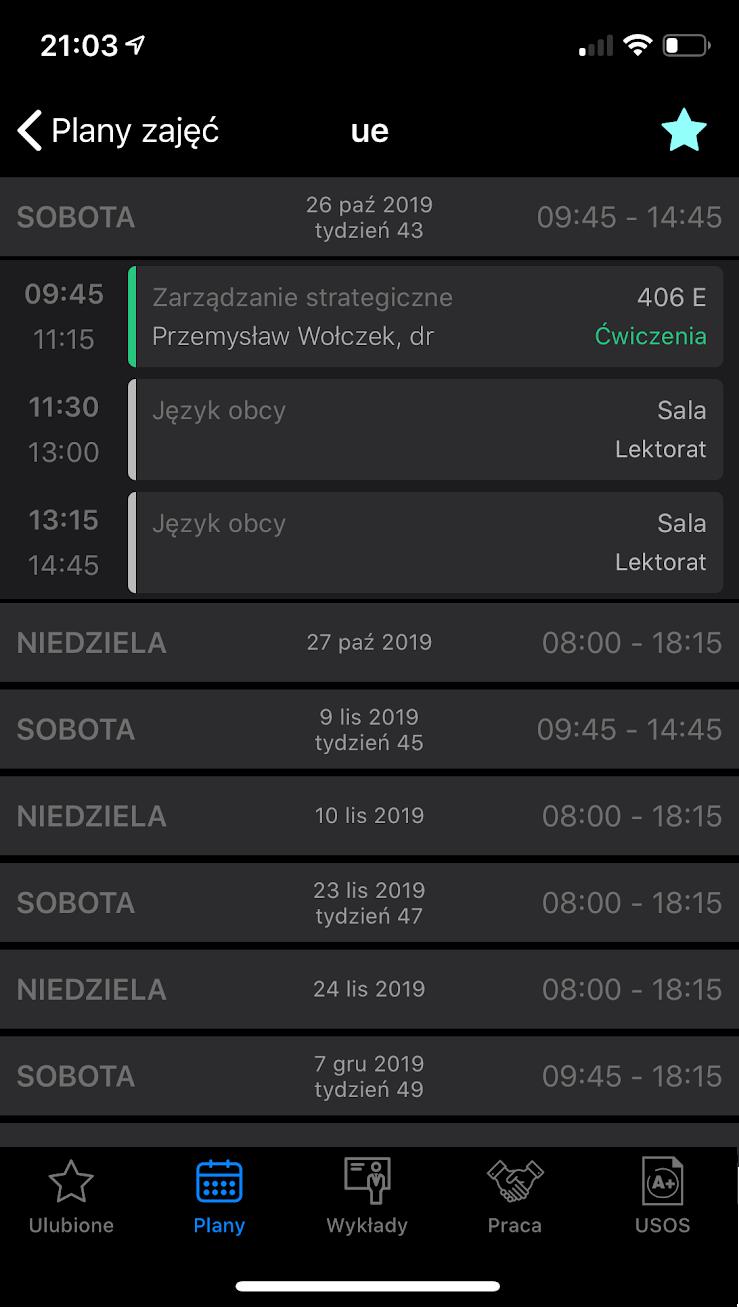
\includegraphics[width=0.425\textwidth]{fig01/kiedy-wyklad.png} \\
    \end{tabular}
    \caption{Interfaces of two mobile applications supporting student service used in Poland: a) Mobilny USOS UW, b) Kiedy wykład} \label{fig:similiar-solutions}
\end{figure}

% TODO - write, that the scope of your system will be defined hereafter

% TODO - write why I chose the topic
% TODO - write about iOS and Android, normally separate applications for both

\section{Objectives and Scope of Thesis}
%  TODO - add more details
The main objective of this thesis is to create a mobile application for both iOS and Android, which will allow users to log in with credentials for their educational institution system, and get access to data published in a student service system. It will store some of the information in a local SQLite database to let users access them offline. Thanks to it, students will be able to see the details when the student services system is down, or they have limited access to the Internet. 
The mobile application will allow logged in students to access:
\begin{itemize}
    \item news feed for a university or faculty,
    \item profile details,
    \item calendar with class details,
    \item list of grades for every semester,
    \item messages and their details,
    \item list of payments.
\end{itemize}

Besides the mobile application, the project requires a server that will act as a service transforming data between two schema-incompatible systems. The app will send a data request to the server using JSON format. This request will be processed there, mapped to a schema of a selected student services system. After it has been mapped, it will be sent to the system requesting data. The last step is to transform the received information and return it to the mobile application in an expected format. The mapping files for universities will be created using the YAML language. This structure will allow the system to be easily expanded with new universities.

\section{Thesis Structure}
% TODO - describe it as a list?
The current chapter acts as an introduction to the topic, provides examples of similar applications created in the past, and explains what the objectives and scope of the thesis are. The second chapter talks about the overall description of the project. It includes a use case diagram with functional as well as non-functional requirements and lists all technologies used during the development of the application. The third part features system architecture along with the database and user interface design. It includes wireframes depicting every screen available in the mobile application. The fourth chapter covers the project implementation. It goes into detail about the database configuration as well as the mobile app and server code. The fifth chapter explains how the applications were tested and provides code snippets. The seventh chapter presents the appearance of the created system and describes the installation and implementation of the program in a production environment. The last chapter summarizes the effects of work and outlines possibilities for the future development of the project.
